% !TEX root = ../main.tex
\section{Introduction}
%-------------------------------------------------------------------------------
A face authentication system verifies the legitimacy of a user by matching a human face, usually in the form of a digital image, against the ones in the database. Such a system has been used in unlocking devices, securing financial payments, and physical access control to critical infrastructures. Due to its non-contact property, face authentication has become the common authentication method compared to other biometric solutions such as fingerprints, especially during the COVID-19 era. However, it has been shown to be vulnerable to spoofing attacks, e.g., 2D replay attack~\cite{chakka2011competition,anjos2011counter,raghavendra2015presentation} that uses a printed photo of the legitimate user.


To prevent such replay attacks, the 3D liveness techniques are exploited to secure the authentication process, and to distinguish the replayed 2D photo by checking its 3D liveness property. Recently, manufacturers such as Apple, Baidu, Tencent, etc.,~\cite{faceid, baidu, tencent} utilize and implement such 3D liveness detection. 
Specifically, it uses a depth camera to obtain the RGB and depth images as the 3D information to determine whether the users are truly present. Thus, the 2D replay attack is impossible to break the 3D face authentication system since the 2D photo lacks the required 3D features, and existing spoofing attacks~\cite{souza2018far, marcel2014handbook} indeed fall short.

\begin{figure}[t]
	\centerline{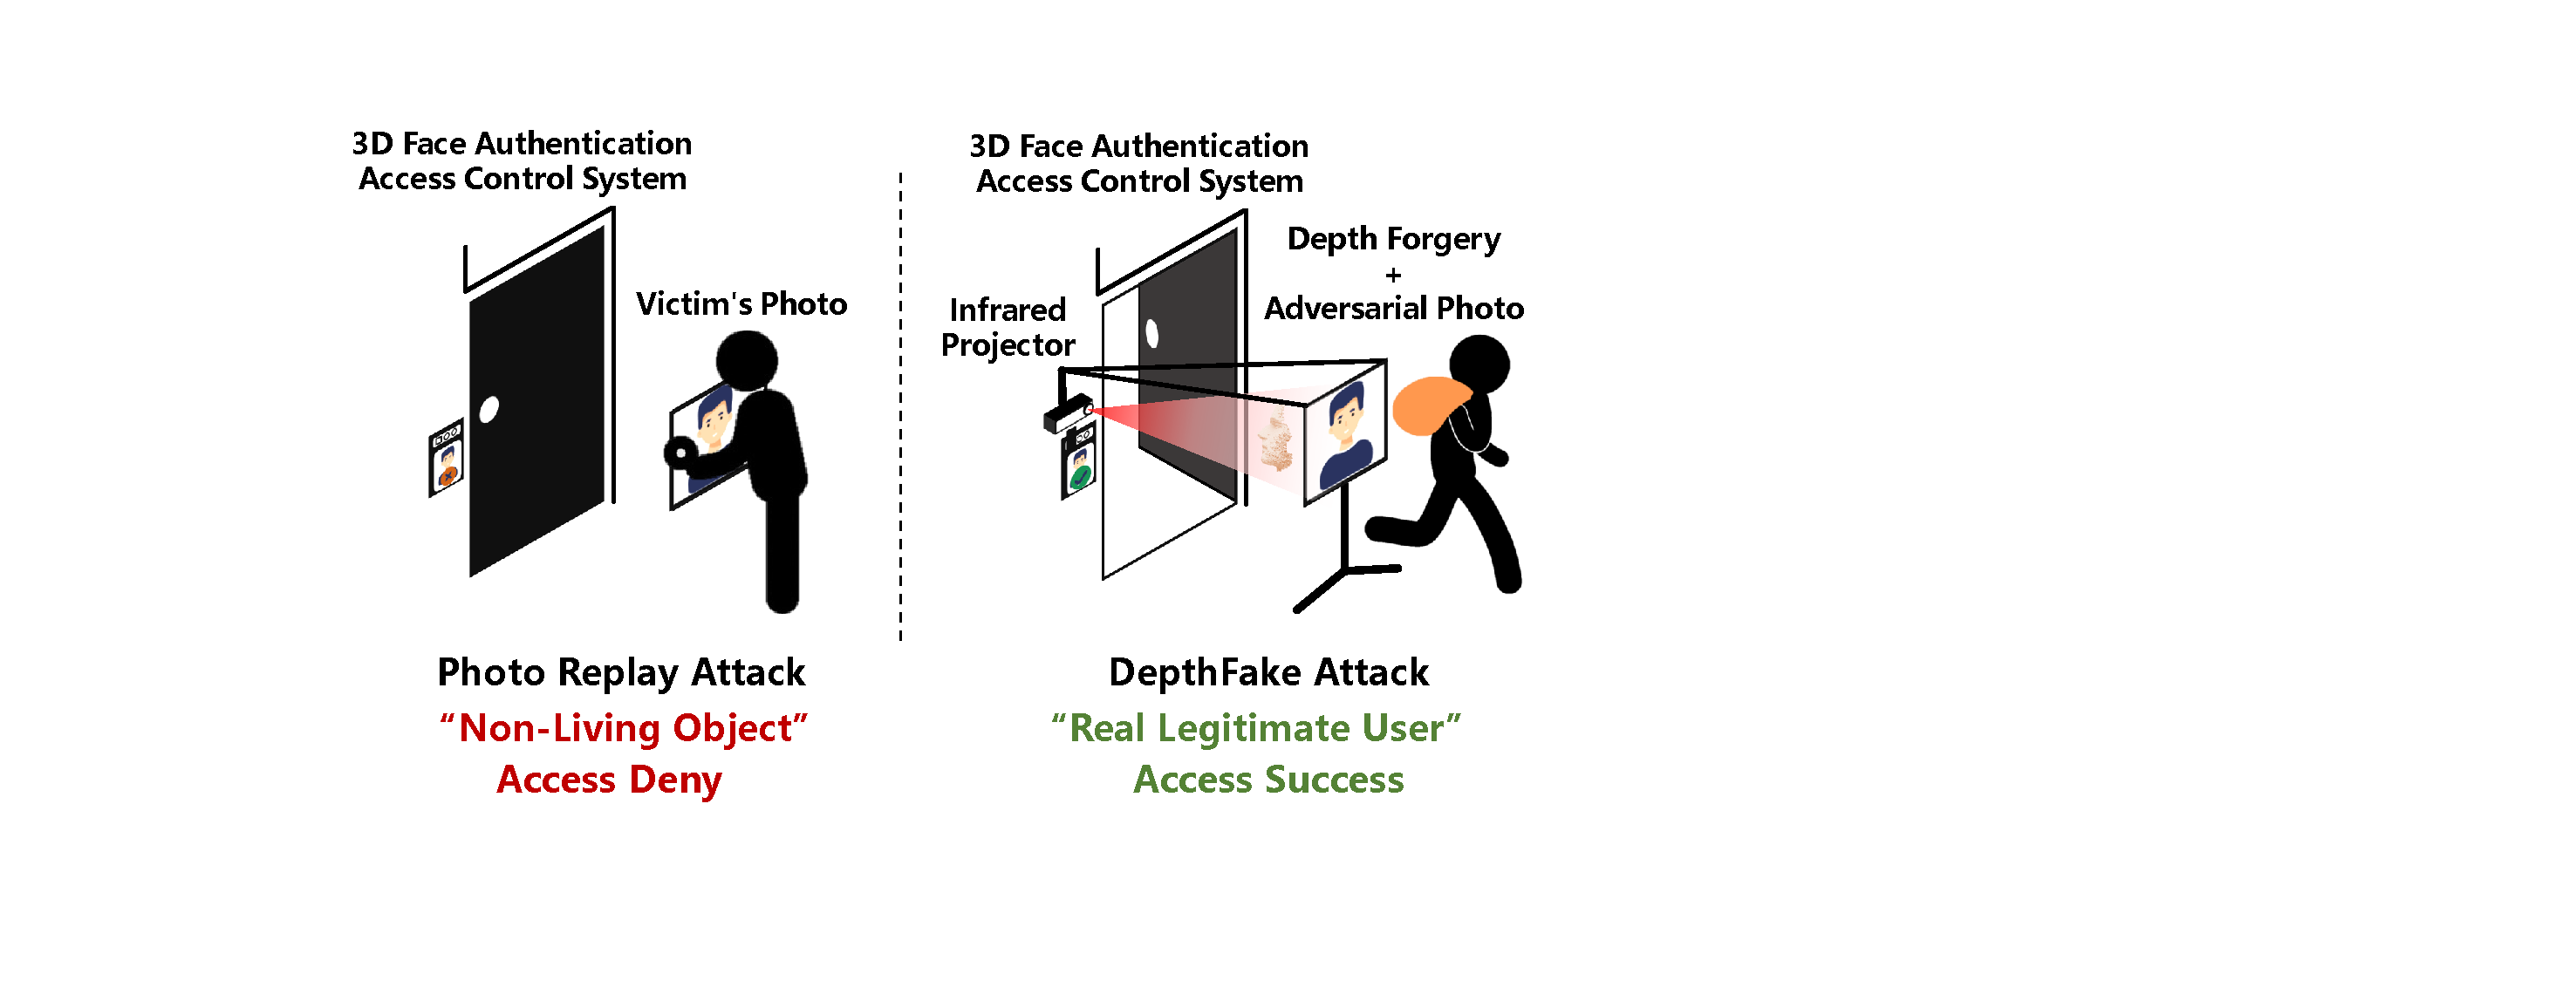
\includegraphics[width = 0.48\textwidth]{figures/intro.pdf}}
	\vspace{-0.1in}
	\caption{The \texttt{DepthFake} attack bypasses the 3D face authentication with liveness detection by projecting the structured light scatter patterns onto the 2D photo of a target victim.}
	\label{intro}
	\vspace{-0.2in}
\end{figure}

In this paper, we seek to answer \emph{``Is it possible to spoof a 3D face authentication system using only a single 2D photo?''}.
The answer is Yes. We find the key to bypassing 3D liveness detection is to forge the depth information and replay it to empower the 2D photo with 3D properties. To this end, we propose the \texttt{DepthFake} attack as shown in Fig.~\ref{intro}. The \texttt{Depthfake} attack first estimates the depth information of the victim from his public 2D photo, then spoofs the depth camera by emitting the infrared pattern which contains the depth information. At last, by aligning the 2D photo with the forgery depth, the \texttt{Depthfake} attack can successfully forge the 3D information of the victim and thus bypass the 3D liveness detection.


However, the design and implementation of \texttt{DepthFake} have several challenges in the real world  against the black-box settings on commercial face authentication systems:
(1) how to obtain the depth information from a single photo?
(2) how to convert the depth information into an infrared pattern that can spoof the structured light depth camera?
(3) how to attack under the black-box systems and physically align the depth information with a 2D photo as uniformed 3D information? 


To address the above challenges, we first propose a CNN-based deep learning model with the weighted loss function to estimate the depth of information from a single photo.
Then, we model the depth measurement process and design the mapping function that can modulate the digital depth image into the desired scatter pattern to spoof the structured light depth camera.
At last, we propose an evolutionary-based RGB adversarial attack method with color calibration, and a face region alignment scheme to form a uniformed RGB-D attack.
We validate the effectiveness of \texttt{DepthFake} attacks on three commercial face authentication systems including Tencent Cloud, Baidu Cloud, and 3DiVi, and a commercial access control device in the real world. \texttt{DepthFake} attack can achieve an overall Depth attack success rate of $78.81\%$ and RGB-D attack success rate of $58.75\%$ under various settings. In summary, our contributions include the points below:
\begin{itemize}	
	\item We identify the vulnerabilities in the 3D liveness detection module of the face authentication system, and propose to spoof a 3D  face authentication system using a single 2D photo.	
	\item We design \texttt{DepthFake},  the first attack in the real world against commercial face authentication systems by projecting the modulated structured light scatter pattern on a printed photo of a target victim.	
	\item We validate the attack effectiveness of  \texttt{DepthFake} on a commercial structured light depth camera (Astra Pro), three commercial face authentication systems (Baidu Cloud, Tencent Cloud, 3DiVi), and one commercial access control device in the real world, and achieve an overall Depth attack success rate of $78.81\%$ and RGB-D attack success rate of $58.75\%$.
\end{itemize}

The \texttt{DepthFake} attack aims to expose the potential threat in 3D face authentication systems and attempts to find a secure authentication solution. Therefore, we propose the following defense methods to prevent such threats:
(1) Randomizing scatter patterns to prevent attackers from forging depth information, which has not been implemented into current depth cameras.
(2) Improving 3D liveness detection models to detect the forgery depth information and adversarial examples.

% First, the single 2D photo captured from the victim's social media do not contain any depth information thus we need to estimate the depth image from it. Second, the estimated depth image shall be modulated into the structured light scatter pattern to spoof the depth camera for generating the forgery depth image. Third, launching attacks both in RGB and depth images to ensure the effectiveness under RGB-D liveness deteciton mode. 


%It seems impossible that a single 2D photo cannot hold the 3D features required to pass the 3D liveness detection and existing spoofing attacks~\cite{souza2018far, marcel2014handbook} indeed fall short. Essentially, we find the key to bypass the 3D liveness detection is to forge the depth information.  
%To this end, we try to use only a single 2D photo to break the 3D face authentication system, and propose the \texttt{DepthFake} attack. 
%
%The \texttt{Depthfake} attack first estimates the depth information of the victim from his public 2D photo, then forges the depth information in the real world by spoofing the structured light depth camera. In this way, a 2D photo is empowered with depth information. In addition, to enhance the attack performance against RGB-D-based liveness detection (i.e., the form of 3D livenss detection), we resort to adversarial example attacks to achieve uniformed spoofing.		


% find that a face authentication system includes a face detection phase, a liveness detection phase, and a face comparison phase, and the three phases work in serial. To bypass the 3D liveness detection, the key is to forge the depth information.

% propose the \texttt{DepthFake} attack, which uses only a single 2D photo to break the 3D face authentication system as shown in Fig.~\ref{intro}. 

%the face authentication systems usually use the RGB-D liveness detection for security purposes, the \texttt{Depthfake} attacks need to be facilitated with the capability of bypassing RGB-based liveness detection such as the edge detection or moiré-pattern check~\cite{yang2014learn, chen2020face, luo2018face}, we resort to the adversarial example attacks and add patterns such as white squares to the printed photos to achieve a flexible spoofing.	
%\texttt{DepthFake} attacks first generate the desired structured-light scatter pattern (normally IR) by measuring the displacements between the reflected and the legitimate ones. Then, the generated structured-light scatter pattern is projected onto the printed photo of the target victim to forge the depth information. 
%In this way, a 2D photo is empowered with the depth information. Our preliminary analysis in Sec.~\ref{sec:preliminary} shows that naively replaying a structured light scatter pattern can generate the depth information but has difficulty in deriving a desired one. In addition, to facilitate \texttt{DepthFake}  attacks with the capability of bypassing RGB-based liveness detection such as the edge detection or moiré-pattern check~\cite{yang2014learn, chen2020face, luo2018face}, we resort to the adversarial example attacks and add patterns such as white squares to the printed photos to achieve a flexible spoofing.	

%First, unlike traditional multi-view depth estimation methods, we obtain the depth information from a single public photo of the victim, which may introduce potential biases.
%Second, the structured light depth camera measures depth information using a specific scatter pattern, thus the depth images shall be converted to the desired scatter pattern.
%Third, the RGB adversarial examples may suffer from the colors shifted and need to align with depth images against the RGB-D liveness detection.

%To prevent 2D replay attacks, manufacturers such as Apple and Microsoft~\cite{faceid} utilize 3D liveness detection techniques to secure the authentication process, which is known as the 3D face authentication system. Specifically, it utilizes a depth camera to obtain the 3D information and identify whether the real user truly present.

% A face authentication system is a technology capable of matching a human face, usually in the form of a digital image, against a database of faces, to authenticate the legitimacy of the user. The enabled services include but are not limited to unlocking devices, securing financial payments, and physical access control to critical infrastructures. Especially, face authentication is regarded as a secure and common authentication method compared to other biometric solutions such as fingerprint authentication due to its non-contact property during the COVID-19 era.

%However, a face authentication system has been shown to be vulnerable to spoofing attacks.
%A naive but efficient idea is to use a printed photo of the legitimate user, which is also known as the 2D replay attack~\cite{chakka2011competition,anjos2011counter,raghavendra2015presentation}. To prevent such 2D replay attacks, face authentication systems nowadays are facilitated with liveness detection techniques. 
%Liveness detection requires users to participate in the authentication process, e.g., shaking their heads, or obtaining their 3D information to ensure they are truly present. In particular, due to the security and user-friendly consideration, the 3D liveness detection is being adopted by more manufacturers, such as Apple, Microsoft, etc. ~\cite{faceid}.